\documentclass[12pt]{article}
%Gummi|065|=)
\usepackage{amsmath, amsfonts, amssymb}
\usepackage[margin=0.5in]{geometry}
\usepackage{xcolor}
%\usepackage{graphicx}
%\usepackage{graphicx}
\newcommand{\off}[1]{}
\DeclareMathSizes{20}{30}{21}{18}

\newcommand{\myhrule}{}

\newcommand{\dash}{
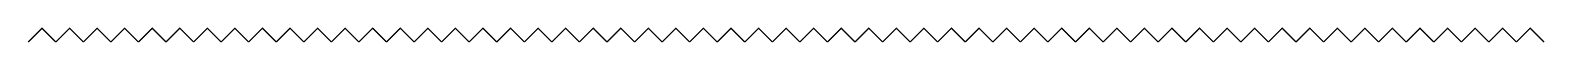
\begin{tikzpicture}[scale=0.35]
\foreach \x in {1,...,55}{
	\draw (\x,-0.25)--(\x+0.5,0.25)--(\x+1,-0.25);
}
\end{tikzpicture}
}

\newcommand{ \sk }{
\begin{tikzpicture}
\draw (0,0)--(18,0);
\end{tikzpicture} \\
}

\usepackage{tikz}

\title{\textbf{ Problem: 8 \& 9 AMC 12A (2016)}}
\author{John D Mangual}
\date{}
\begin{document}

\fontfamily{qag}\selectfont \fontsize{25}{32}\selectfont

\maketitle

\noindent  \textbf{Problem} What s the area of the shaded region of the given $8 \times 5$ rectangle ? \\ \\
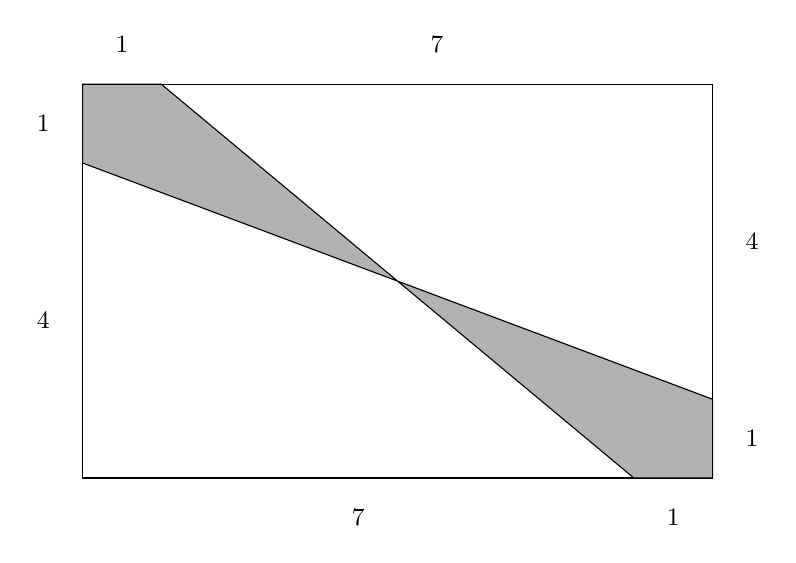
\begin{tikzpicture}
\draw (0,0)--(8,0)--(8,5)--(0,5)--cycle;
\draw[fill=black!30!white] (7,0)--(8,0)--(8,1)--(0,4)--(0,5)--(1,5)--cycle;
\node at (7.5,-0.5) {\small 1};
\node at (3.5,-0.5) {\small 7};
\node at (8.5, 0.5) {\small 1};
\node at (8.5, 3) {\small 4};
\node at (4.5, 5.5) {\small 7};
\node at (0.5, 5.5) {\small 1};
\node at (-0.5,4.5) {\small 1};
\node at (-0.5, 2) {\small 4};
\end{tikzpicture} \\
(A) $4 \frac{3}{4}$ \; (B) $5$ \; (C) $5 \frac{1}{4}$\; (D) $6 \frac{1}{2}$ \; (E) $8$

\begin{tikzpicture}
\draw (0,0)--(18,0);
\end{tikzpicture} \\
A lot of things come to mind $\sqrt{1^2 + 1^2} = \sqrt{2}$ or $\sqrt{4^2 + 7^2} = \sqrt{65}$ none of these look very useful.  

\newpage \noindent I considered this rhombus for a while.  There really is not much time.\\
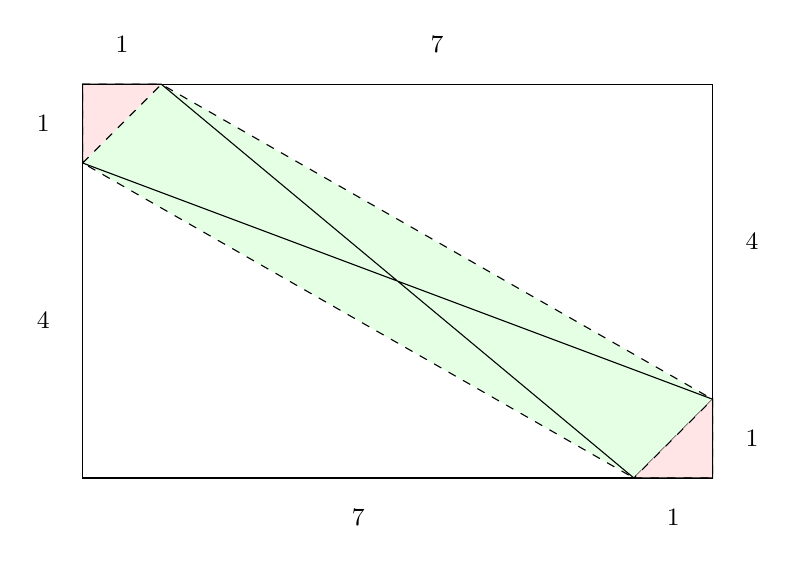
\begin{tikzpicture}
\draw (0,0)--(8,0)--(8,5)--(0,5)--cycle;

\draw[fill=green!10!white, dashed] (0,4)--(1,5)--(8,1)--(7,0)--cycle;
\draw[fill=red!10!white,dashed] (0,4)--(1,5)--(0,5)--cycle;
\draw[fill=red!10!white, dashed] (7,0)--(8,0)--(8,1)--cycle;
\draw (7,0)--(8,0)--(8,1)--(0,4)--(0,5)--(1,5)--cycle;
\node at (7.5,-0.5) {\small 1};
\node at (3.5,-0.5) {\small 7};
\node at (8.5, 0.5) {\small 1};
\node at (8.5, 3) {\small 4};
\node at (4.5, 5.5) {\small 7};
\node at (0.5, 5.5) {\small 1};
\node at (-0.5,4.5) {\small 1};
\node at (-0.5, 2) {\small 4};
\end{tikzpicture} \\
I am guess the shaded region is the sum of the two {\color{red!50!white} red} triangles ($A=1$) and half of the {\color{green!50!white} green} rhombus (which is slanted).
$$ A = \frac{1}{2} \bigg(8 \times 5 - \big( 1 \times 1 + 4 \times 7 \big)\bigg) + 1 = 6 \frac{1}{2}$$
Is there any way to corroborate choice \textbf{(C)}?

\newpage

\noindent Here is a ``Japanese" or \textbf{sangaku} type of solution, involvng the area of the triangle. \\ \\
Just cut into 4 pieces and just use $A = \frac{1}{2}bh$:\\
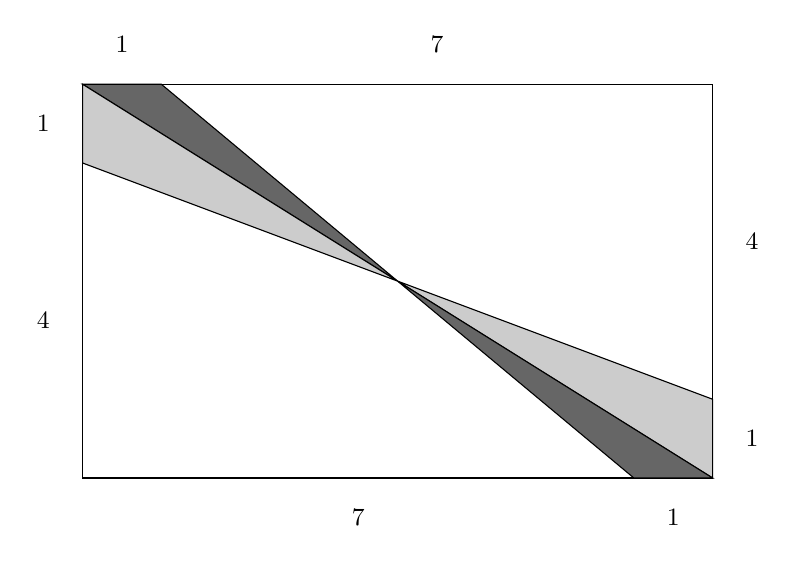
\begin{tikzpicture}
\draw (0,0)--(8,0)--(8,5)--(0,5)--cycle;


\draw[fill=black!60!white] (0,5)--(4,2.5)--(1,5)--cycle;
\draw[fill=black!20!white] (0,5)--(4,2.5)--(0,4)--cycle;
\draw[fill=black!20!white] (8,0)--(8,1)--(4,2.5)--cycle;
\draw[fill=black!60!white] (8,0)--(4,2.5)--(7,0)--cycle;

\node at (7.5,-0.5) {\small 1};
\node at (3.5,-0.5) {\small 7};
\node at (8.5, 0.5) {\small 1};
\node at (8.5, 3) {\small 4};
\node at (4.5, 5.5) {\small 7};
\node at (0.5, 5.5) {\small 1};
\node at (-0.5,4.5) {\small 1};
\node at (-0.5, 2) {\small 4};
\end{tikzpicture} \\
The two black triangles have area:
$$ A_1 + A_2 = \bigg(1 \times \frac{4+1}{2} \bigg)+ \bigg(1 \times \frac{7+1}{2} \bigg) = 6 \,\tfrac{1}{2}$$
This again is choice \textbf{(C)}. \newpage

\noindent \textbf{Problem} The five small shaded squares inside this unit square are congruent and have disjoint interiors.  The midpoint of each side of the middle square coincides with one of the vertices of the other four small squares shown.  The common side length is $\frac{a - \sqrt{2}}{b}$ where $a$ and $b$ are positive integers what is $a+b$?\\

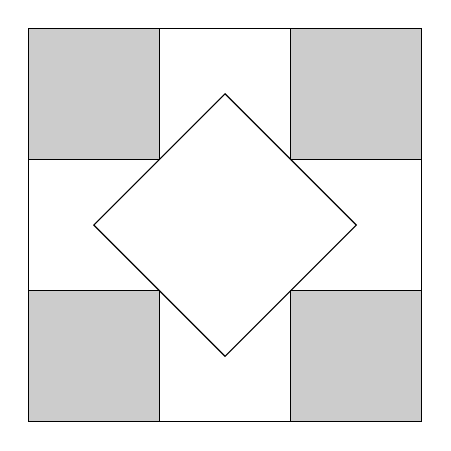
\begin{tikzpicture}[scale=5]
\draw (0,0)--(1,0)--(1,1)--(0,1)--cycle;
\draw[fill=black!20!white] (0,0)--(1/3,0)--(1/3,1/3)--(0,1/3)--cycle;
\draw[fill=black!20!white] (1,0)--(2/3,0)--(2/3,1/3)--(1,1/3)--cycle;
\draw[fill=black!20!white] (0,1)--(1/3,1)--(1/3,2/3)--(0,2/3)--cycle;
\draw[fill=black!20!white] (1,1)--(2/3,1)--(2/3,2/3)--(1,2/3)--cycle;
\draw (1/2, 1-1/6)--(1/6, 1/2)--(1/2, 1/6)--( 1-1/6, 1/2)--cycle;
\end{tikzpicture}
This diagram looks convincing.  If I could draw it correctly, I would immediately have you the answer. \\ \\ If the shaded squares have side-length $a$ the midpoints of the white square is $(a,a)$ and the corners are at $( \frac{1}{2}, 2a - \frac{1}{2}), (2a - \frac{1}{2} , \frac{1}{2}) $ etc. so the area is:
$$ A = 2 \times (2a-1)^2  = a^2 $$
When does $\sqrt{2}(2a-1)=a$ ? It happens when 
$$ a = \frac{\sqrt{2}}{2 \sqrt{2}-1}= \frac{\sqrt{2}(2\sqrt{2}+1)}{7} = \frac{4 + \sqrt{2}}{7}$$
and $\boxed{4+7=11}$.  This is choice \textbf{(E)}
\end{document}